%
% teil3.tex -- Beispiel-File für Teil 3
%
% (c) 2020 Prof Dr Andreas Müller, Hochschule Rapperswil
%
% !TEX root = ../../buch.tex
% !TEX encoding = UTF-8
%
\section{Schallausbreitung bei Überschallflugzeugen
\label{schall:section:teil3}}
\kopfrechts{Teil 3}

In diesem Abschnitt wenden wir die in den vorherigen Abschnitten
beschriebenen Konzepte an, um die Schallausbreitung bei einem
Flugzeug im Überschall zu beschreiben.
Ziel ist es, die Entstehung des Überschallknalls herzuleiten und Strategien
zur Reduktion desselben zu verstehen.
Dabei betrachten wir eine ideale Situation, in der das Flugzeug als
Punktquelle modelliert wird.

Wir betrachten ein Flugzeug, das sich mit konstanter Geschwindigkeit
$V>0$ entlang einer horizontalen Bahn auf der Höhe $z=z_a$ über
dem Grund $z=0$ bewegt.
Das Medium sei ein ideales Gas mit örtlich variabler Temperatur
$T(z)$ aber ohne Wind, sodass
\begin{equation}
    c(z) \;=\; \sqrt{\kappa R_S\,T(z)} ,
    \label{eq:c-of-z}
\end{equation}
gilt. Hier ist $c(z)$ die lokale Schallgeschwindigkeit, $R_S = \frac{R}{M}$
die Massenangepasste Gaskonstante und $M$ die auf der Höhe $z$ herrschende
molare Masse des Mediums.
In der Fliegerei wird die Geschwindigkeit des Flugzeugs oft über die
dimensionslose \emph{Machzahl} \textit{Ma} angegeben:
\begin{equation}
    \textit{Ma}(z) \;=\; \frac{V}{c(z)},
    \label{eq:mach-number}
\end{equation}
wobei $\textit{Ma}<1$ Unterschall, $\textit{Ma}=1$ Schallgeschwindigkeit
und $\textit{Ma}>1$ Überschall bezeichnet.
Der Effekt des Schall- oder Machkegels, welcher durch den Dopplereffekt
beschrieben wird, ist im Bild \ref{fig:schall:mach-zones} visualisiert.

\begin{figure}
    \centering
    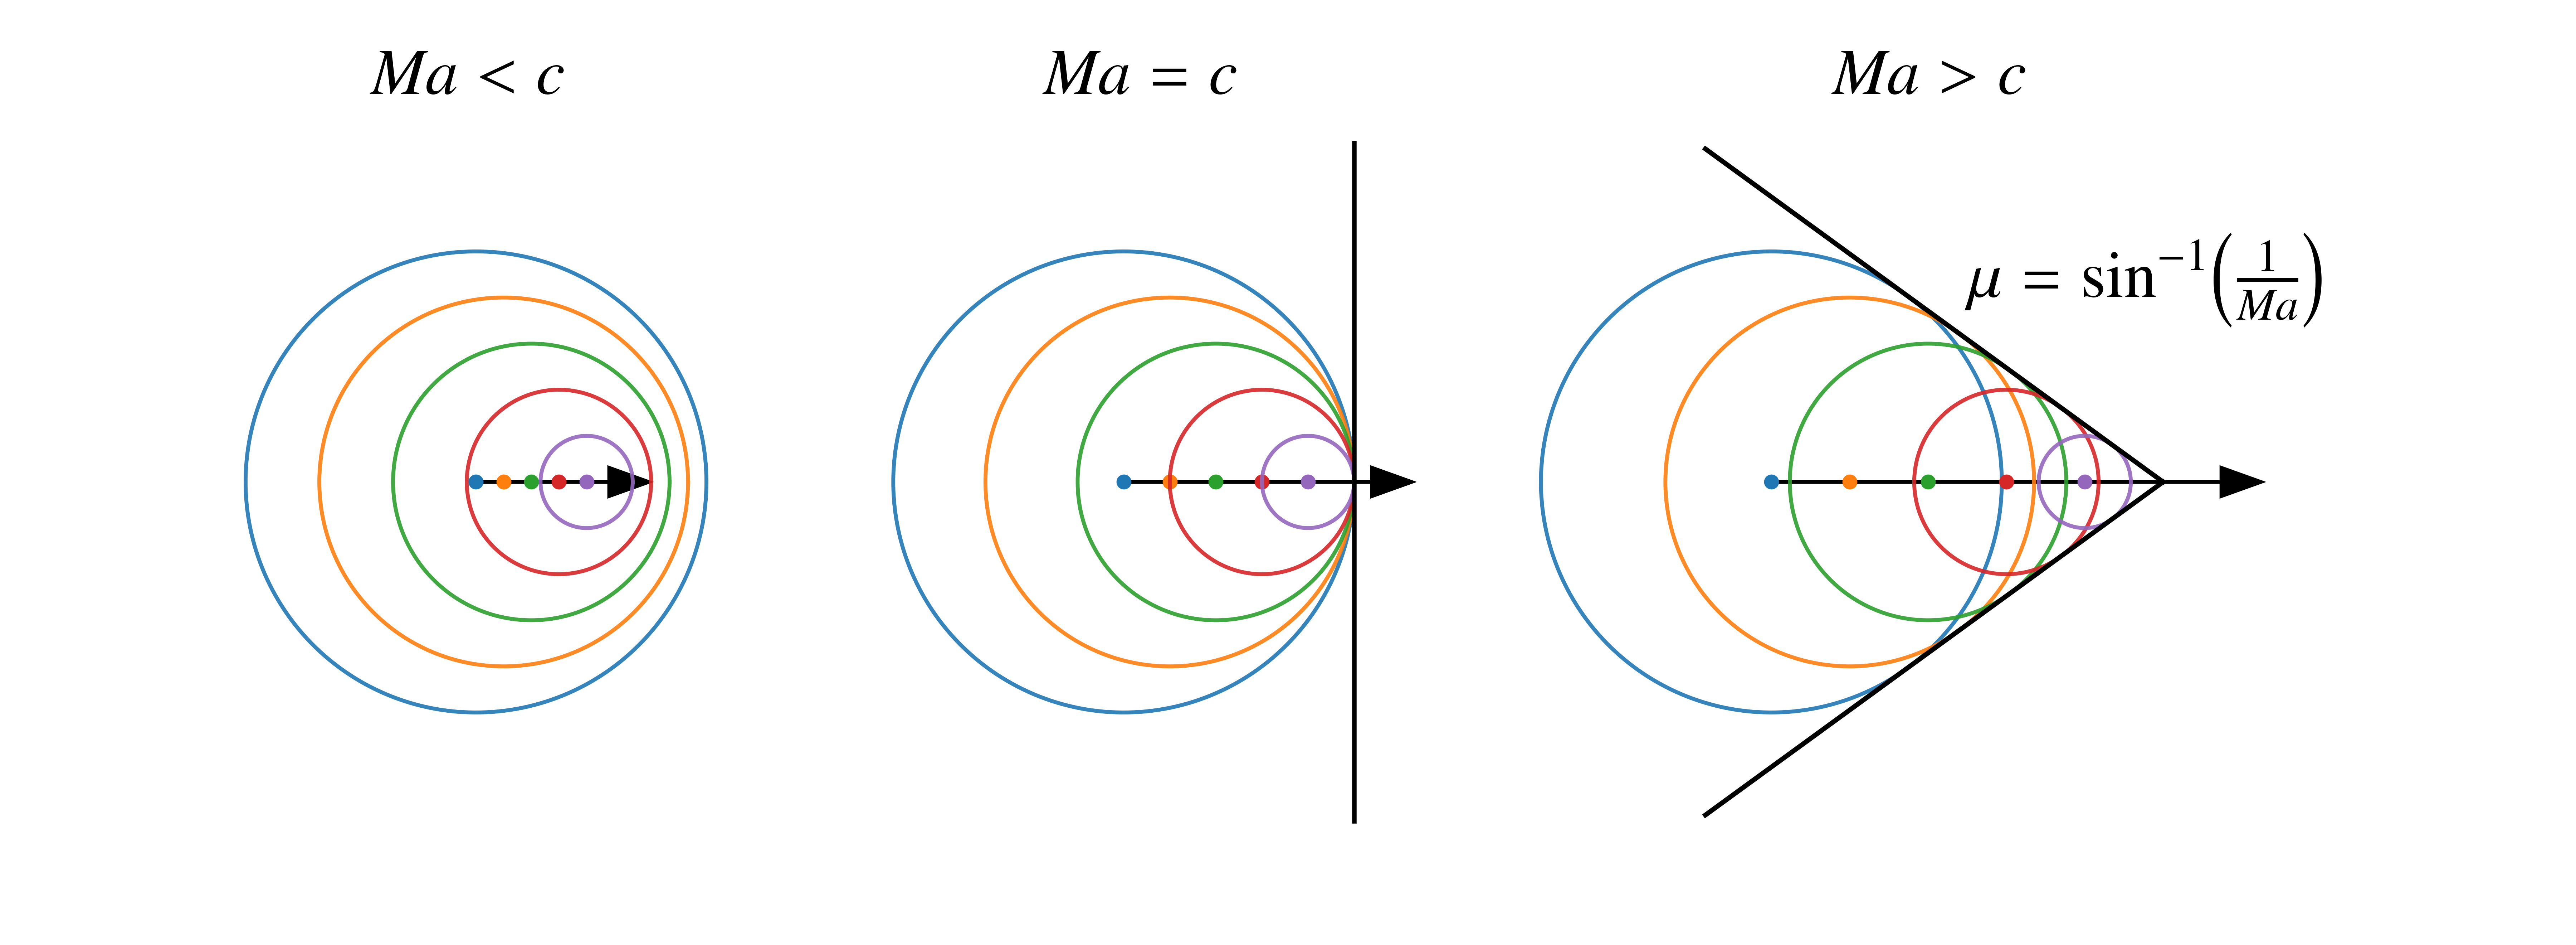
\includegraphics[width=\textwidth]{papers/schall/figures/mach_doppler_triptych_offsets.png}
    \caption{Dopplereffekt bei Unterschall, Schallgeschwindigkeit und Überschall.
    Für die Schallgeschwindigkeit und den Überschall ist zusätzlich der
    Machkegel mit dem Machwinkel $\mu$ eingezeichnet.}
    \label{fig:schall:mach-zones}
\end{figure}
Das vom Flugzeug erzeugte Schallereignis bewegt sich mit Geschwindigkeit $V$
mit dem Flugzeug, der Schall breitet sich aber mit $c(z)$ aus.
Diese ist jedoch nicht überall gleich: je dichter ein Medium ist, desto
höher ist die Schallgeschwindigkeit, was im
Kapitel~\ref{schall:subsection:atmos-scenarios} aufgezeigt wird.
Tritt die vom Überschall erzeugte Schockwelle in eine Region mit höherer
Schallgeschwindigkeit ein sodass $V<c(z)$ gilt, so wird die Schockwelle
nach oben abgelenkt und kann sich nicht mehr bis zum Boden ausbreiten.
Tritt hingegen eine Schallwelle in eine Region mit niedrigerer
Schallgeschwindigkeit ein, sodass $V>c(z)$ gilt, so wird eine Schockwelle
entstehen, die sich bis zum Boden ausbreiten kann.

Wenn $V \gg c(z)$ ist, wie zum Beispiel beim Flug der Concorde mit Mach
$2.2 \gg c$, dann spielen die Varitionen von $c(z)$ keine grosse Rolle.
Wenn aber $V$ nahe bei $c(z)$ ist, dann kommt es zu merklichen Einflüssen,
die dazu genutzt werden, den Überschallknall abzuschwächen oder zu
unterdrücken, was im Kapitel~\ref{schall:section:boom} analysiert wird.

\subsection{Lokaler Machwinkel und Emissionsrichtung}
In einem homogenem Medium bildet sich der Machkegel mit Halbwinkel
\begin{equation}
    \mu \;=\; \arcsin\!\Big(\frac{1}{\textit{Ma}}\Big).
\end{equation}
In einem geschichteten Medium setzt man diesen \emph{lokal} an der
Emissionshöhe $z_a$, auf welcher das Flugzeug fliegt, an:
\begin{equation}
    \mu_a \;:=\; \arcsin\!\Big(\frac{1}{\textit{Ma}(z_a)}\Big)
    \;=\; \arcsin\!\Big(\frac{c(z_a)}{V}\Big) .
    \label{eq:local-mach-angle}
\end{equation}
Der Rand des Machkegels wird oft als Machrand bezeichnet, welcher im
vertikalen Schnitt $(x,z)$ durch akustische Strahlen begrenzt ist.
Dies nennt man die \emph{geometrische Akustik}.

\paragraph{Akustische Strahlen.}
Seien $\tau(\mathbf{x})=\mathrm{const.}$ die \emph{Wellenfronten}, visualisiert
als Kreise in der Abbildung \ref{fig:schall:mach-zones}.
Die akustischen Strahlen sind ihre \emph{Normalen}; formal verlaufen sie
in Richtung des Gradienten $\nabla\tau$ und beschreiben die lokale
Ausbreitungsrichtung:
\[
    \dot{\mathbf{x}}(s)\ \parallel\ \nabla\tau(\mathbf{x}),\qquad
    \text{Strahl}\ \perp\ \text{Wellenfront}.
\]
In einem \emph{homogenen} Medium sind Strahlen \emph{Geraden}.
Für einen \emph{bewegten Punktstrahler}, wie zum Beispiel ein Flugzeug,
sind die Wellenfronten die Kreise $r=c\,\tau$ um die jeweiligen Emissionsorte
$x=V(t-\tau)$; die Strahlen an jedem Punkt der Front zeigen radial auf den Emissionsort.

\paragraph{Einhüllende (Machrand) vs.\ Strahlen.}
Der \emph{Machrand} ist die \emph{Einhüllende} der expandierenden Wellenfronten:
die Menge aller \emph{Tangentialpunkte} zwischen den Kreisen und einer Kurve.
An \emph{Einhüllendenpunkten} gilt: \emph{Strahl $\perp$ Einhüllende},
denn der Strahl ist normal auf die Wellenfront.
Die Einhüllende ist dort tangential an die Wellenfront.

\begin{itemize}
\item \textbf{Unterschall} ($\textit{Ma}<1$):
Es existiert \emph{keine} Einhüllende; die Kreise überlappen, Strahlen
sind radial zu ihren Emissionszentren und es entsteht kein Machrand.

\item \textbf{Schallnah} ($\textit{Ma}=1$):
Die Einhüllende degeneriert zu einer \emph{Geraden} senkrecht zur Flugrichtung,
was zu einer „vertikale“ Linie in der Visualisierung \ref{fig:schall:mach-zones} führt.
Die Strahlen an den Berührungspunkten sind \emph{orthogonal} zu dieser Linie,
also parallel zur Flugrichtung.
Sie liegen nicht auf der Einhüllenden, sondern stehen \emph{senkrecht} zu ihr.

\item \textbf{Überschall} ($\textit{Ma}>1$):
Die Einhüllende besteht aus zwei \emph{Geraden} mit Halbwinkel $\mu_a$ zur Flugrichtung.
Dies sind die \emph{Generatoren} des Machkegels, was der Mach-Rand ist,
und nicht die Strahlen selbst.
Die Strahlen in den Berührungspunkten stehen \emph{senkrecht} zu
diesen Linien und zeigen radial zu ihren jeweiligen Emissionszentren;
sie verlaufen \emph{nicht} entlang der Machlinien.
\end{itemize}

\subsection{Strahlen in geschichtetem Medium}
Für isotrope, ruhende Medien mit $c=c(z)$ liefert die geometrische
Akustik eine Snell-ähnliche Invariante:
\begin{equation}
    \frac{\sin\theta(z)}{c(z)} \;=\; \text{const} \;=:\; K ,
    \label{eq:snell-acoustics}
\end{equation}
wobei $\theta(z)$ der Winkel des Strahls relativ zur Horizontalen ist.
Wählt man als Anfangsbedingung den lokalen Machwinkel an $z=z_a$,
also $\theta(z_a)=\mu_a$, dann folgt aus \eqref{eq:snell-acoustics}
\[
    K \;=\; \frac{\sin\mu_a}{c(z_a)} \;=\; \frac{1/\textit{Ma}(z_a)}{c(z_a)} \;=\; \frac{1}{V}.
\]
Damit ist für Mach-Strahlen die Invariante schlicht
\begin{equation}
    K \;=\; \frac{1}{V}.
    \label{eq:K-equals-1-over-V}
\end{equation}

Mit $\tan\theta = \dfrac{dz}{dx}$, $\sin\theta = K\,c(z)$ und
$\cos\theta = \sqrt{1 - \sin^2\theta}$,
erhält man aus trigonometischen Identitäten
\begin{equation}
    \frac{dz}{dx} \;=\; \frac{\sin\theta(z)}{\cos\theta(z)} \;=\;
    \frac{K\,c(z)}{\sqrt{1 - K^2 c^2(z)}}.
\end{equation}
Einsetzen von \eqref{eq:K-equals-1-over-V} liefert die
\emph{Bahn-Differentialgleichung} der Mach-Ränder:
\[
    \quad
    \frac{dz}{dx} \;=\; \frac{c(z)/V}{\sqrt{1 - \big(c(z)/V\big)^2}}
    \;=\; \frac{1}{\sqrt{\frac{V^2}{c^2(z)} - 1}}
    \quad
\]
oder äquivalent
\begin{equation}
    \quad
    \frac{dx}{dz} \;=\; \sqrt{\frac{V^2}{c^2(z)} - 1}
    \quad
    \label{eq:ray-ode-inverse}
\end{equation}
mit Anfangsbedingung $x(z_a)=0$ senkrecht unter dem Flugzeug.
Die Lösungen von \eqref{eq:ray-ode-inverse} geben die gekrümmten Stossränder
im $(x,z)$-Schnitt.
Die \emph{Bedingung für reale Strahlen} ist $V>c(z)$ entlang der Bahn;
wo $V=c(z)$ wird, existiert ein \emph{Wendepunkt}/
\emph{kritische Höhe}, die Evaneszenz.
Dies wird in Kapitel~\ref{schall:subsection:atmos-scenarios} genauer analysiert.

\subsection{Bodenaufprall (Sonic-Boom-Carpet)}
Die horizontale Entfernung vom Lotpunkt des Flugzeugs bis zum
Aufprallpunkt eines Strahls am Boden ($z=0$) ergibt sich durch
Integration von \eqref{eq:ray-ode-inverse}:
\begin{equation}
    \quad
    x_g \;=\; \int_{0}^{z_a} \sqrt{\frac{V^2}{c^2(\zeta)} - 1}\;\, d\zeta,
    \qquad \text{sofern } V>c(\zeta) \text{ für } \zeta\in[0,z_a].
    \quad
    \label{eq:ground-range}
\end{equation}
In einer Schicht mit $V\le c(\zeta)$, wird der Mach-Rand kontinuierlich
nach oben abgelenkt und die Schockwelle breitet sich nicht weiter aus,
was zu Schattenzonen am Boden führt.

\subsection{Atmosphären-Szenarien}\label{schall:subsection:atmos-scenarios}
Wir modellieren $T(z)$ stückweise linear und mit trockener
Standardatmosphäre ohne Wind, woraus $c(z)$ via \eqref{eq:c-of-z} folgt.

\paragraph{Normale Lage (Temperatur nimmt mit Höhe ab).}
Es gelte
\begin{equation}
    T(z) \;=\; T_0 - Lz \quad (L>0),
    \qquad
    c(z) \;=\; \sqrt{\kappa R\,(T_0 - Lz)} .
    \label{eq:normal-lapse}
\end{equation}
Da $c$ mit $z$ \emph{abnimmt}, sind höhere Schichten akustisch
``langsamer''; Strahlen werden zum \emph{langsameren} Bereich hin
gebogen, d.\,h.\ \emph{nach oben}.
Damit nimmt $x_g$ in \eqref{eq:ground-range} ab, was sich in einem anheben
der Strahlen wiederspiegelt, und es können \emph{Bodenschatten}
entstehen, wenn in Bodennähe $V\lesssim c(0)$ ist.

\paragraph{Inversionslage (Temperatur nimmt mit Höhe zu, z.\,B.
nächtliche Bodeninversion über einem kalten Boden).}
Es gelte
\begin{equation}
    T(z) \;=\; T_0 + L_{I} z \quad (L_{I}>0),
    \qquad
    c(z) \;=\; \sqrt{\kappa R\,(T_0 + L_{I} z)} .
    \label{eq:inversion}
\end{equation}
Nun \emph{nimmt $c$ mit $z$ zu}; höhere Schichten sind akustisch ``schneller''.
Strahlen biegen daher \emph{nach unten} und werden zum Boden zurückgeführt.
Dadurch wächst $x_g$ in \eqref{eq:ground-range} und der Überschall
kann \emph{weiter} getragen werden, was zu weniger oder bis zu keine
Schattierung am Boden führt.

\paragraph{Wendepunkt und Bodenschatten (kein Bodentreffer).}
Tritt irgendwo im Intervall $[0,z_a]$ ein Bereich auf, in dem
$V\le c(\zeta)$ gilt, so existiert eine
\emph{kritische Höhe} $z_\ast\in(0,z_a]$ mit
\begin{equation}
    c(z_\ast)=V.
    \label{eq:turning-def}
\end{equation}
Dieser kritische Punkt ist ein \emph{Wendepunkt} des akustischen Ausbreitungsstrahls.
Aus der Strahlgleichung \eqref{eq:ray-ode-inverse} folgt, dass der
Integrand für $z\to z_\ast$ gegen $0$ geht und für $z<z_\ast$ imaginär würde.
Der Strahl besitzt bei $z=z_\ast$ eine \emph{horizontale Tangente} und kehrt um;
er kann die Schicht $z<z_\ast$ nicht durchdringen.
Die maximale horizontale Ausbreitung bis zum Wendepunkt ist
\begin{equation}
    x_{\mathrm{turn}}
    \;=\; \int_{z_\ast}^{z_a} \sqrt{\frac{V^2}{c^2(\zeta)}-1}\;d\zeta,
    \label{eq:x-turn}
\end{equation}
die \emph{Bodenentfernung} \eqref{eq:ground-range} ist hingegen \emph{nicht}
definiert, da $z=0$ nicht erreichbar ist.
Der Bereich unterhalb der Wendeschicht $z<z_\ast$ liegt somit in einer
\emph{Schattenzone}, indem man keinen Schall des Flugzeugs höhren kann.

Für streng monotone Profile entscheidet die einfache Bedingung
\begin{equation}
    \text{Bodentreffer existiert} \;\Leftrightarrow\; V>c(z)\quad\forall\,z\in[0,z_a].
    \label{eq:ground-hit-condition}
\end{equation}


% \begin{figure}
% \centering
% \begin{minipage}[t]{0.5\textwidth}
%   \centering
%   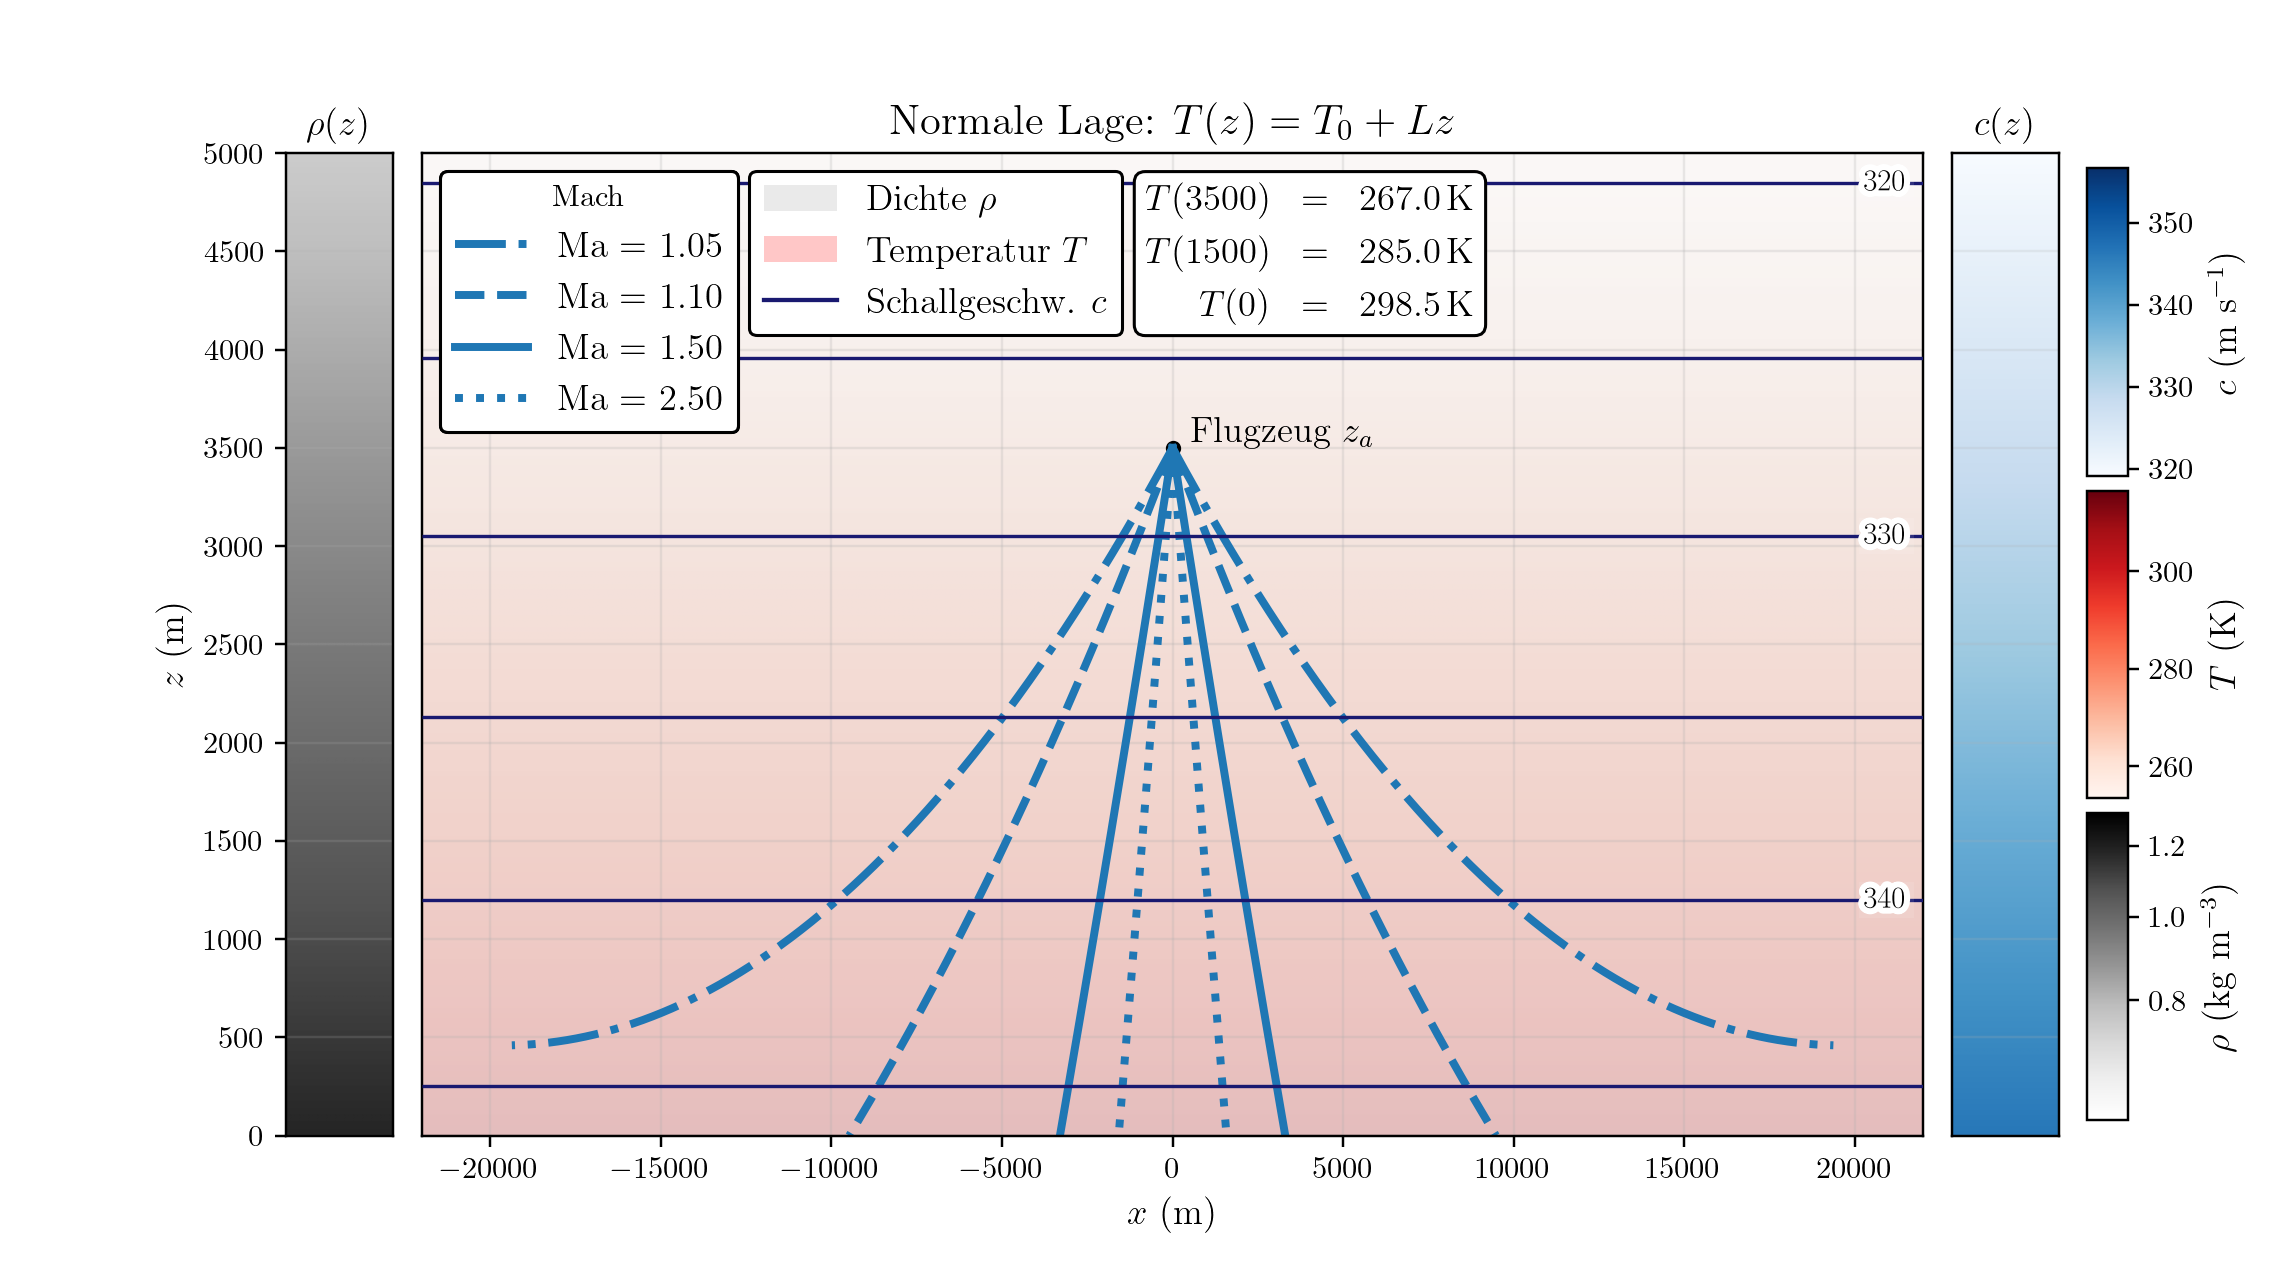
\includegraphics[width=0.9\linewidth]{papers/schall/figures/normal_sidepanels.png}
%   \captionof{subfigure}{Normale Lage}
%   \label{fig:norm}
% \end{minipage}\hfill
% \begin{minipage}[t]{0.5\textwidth}
%   \centering
%   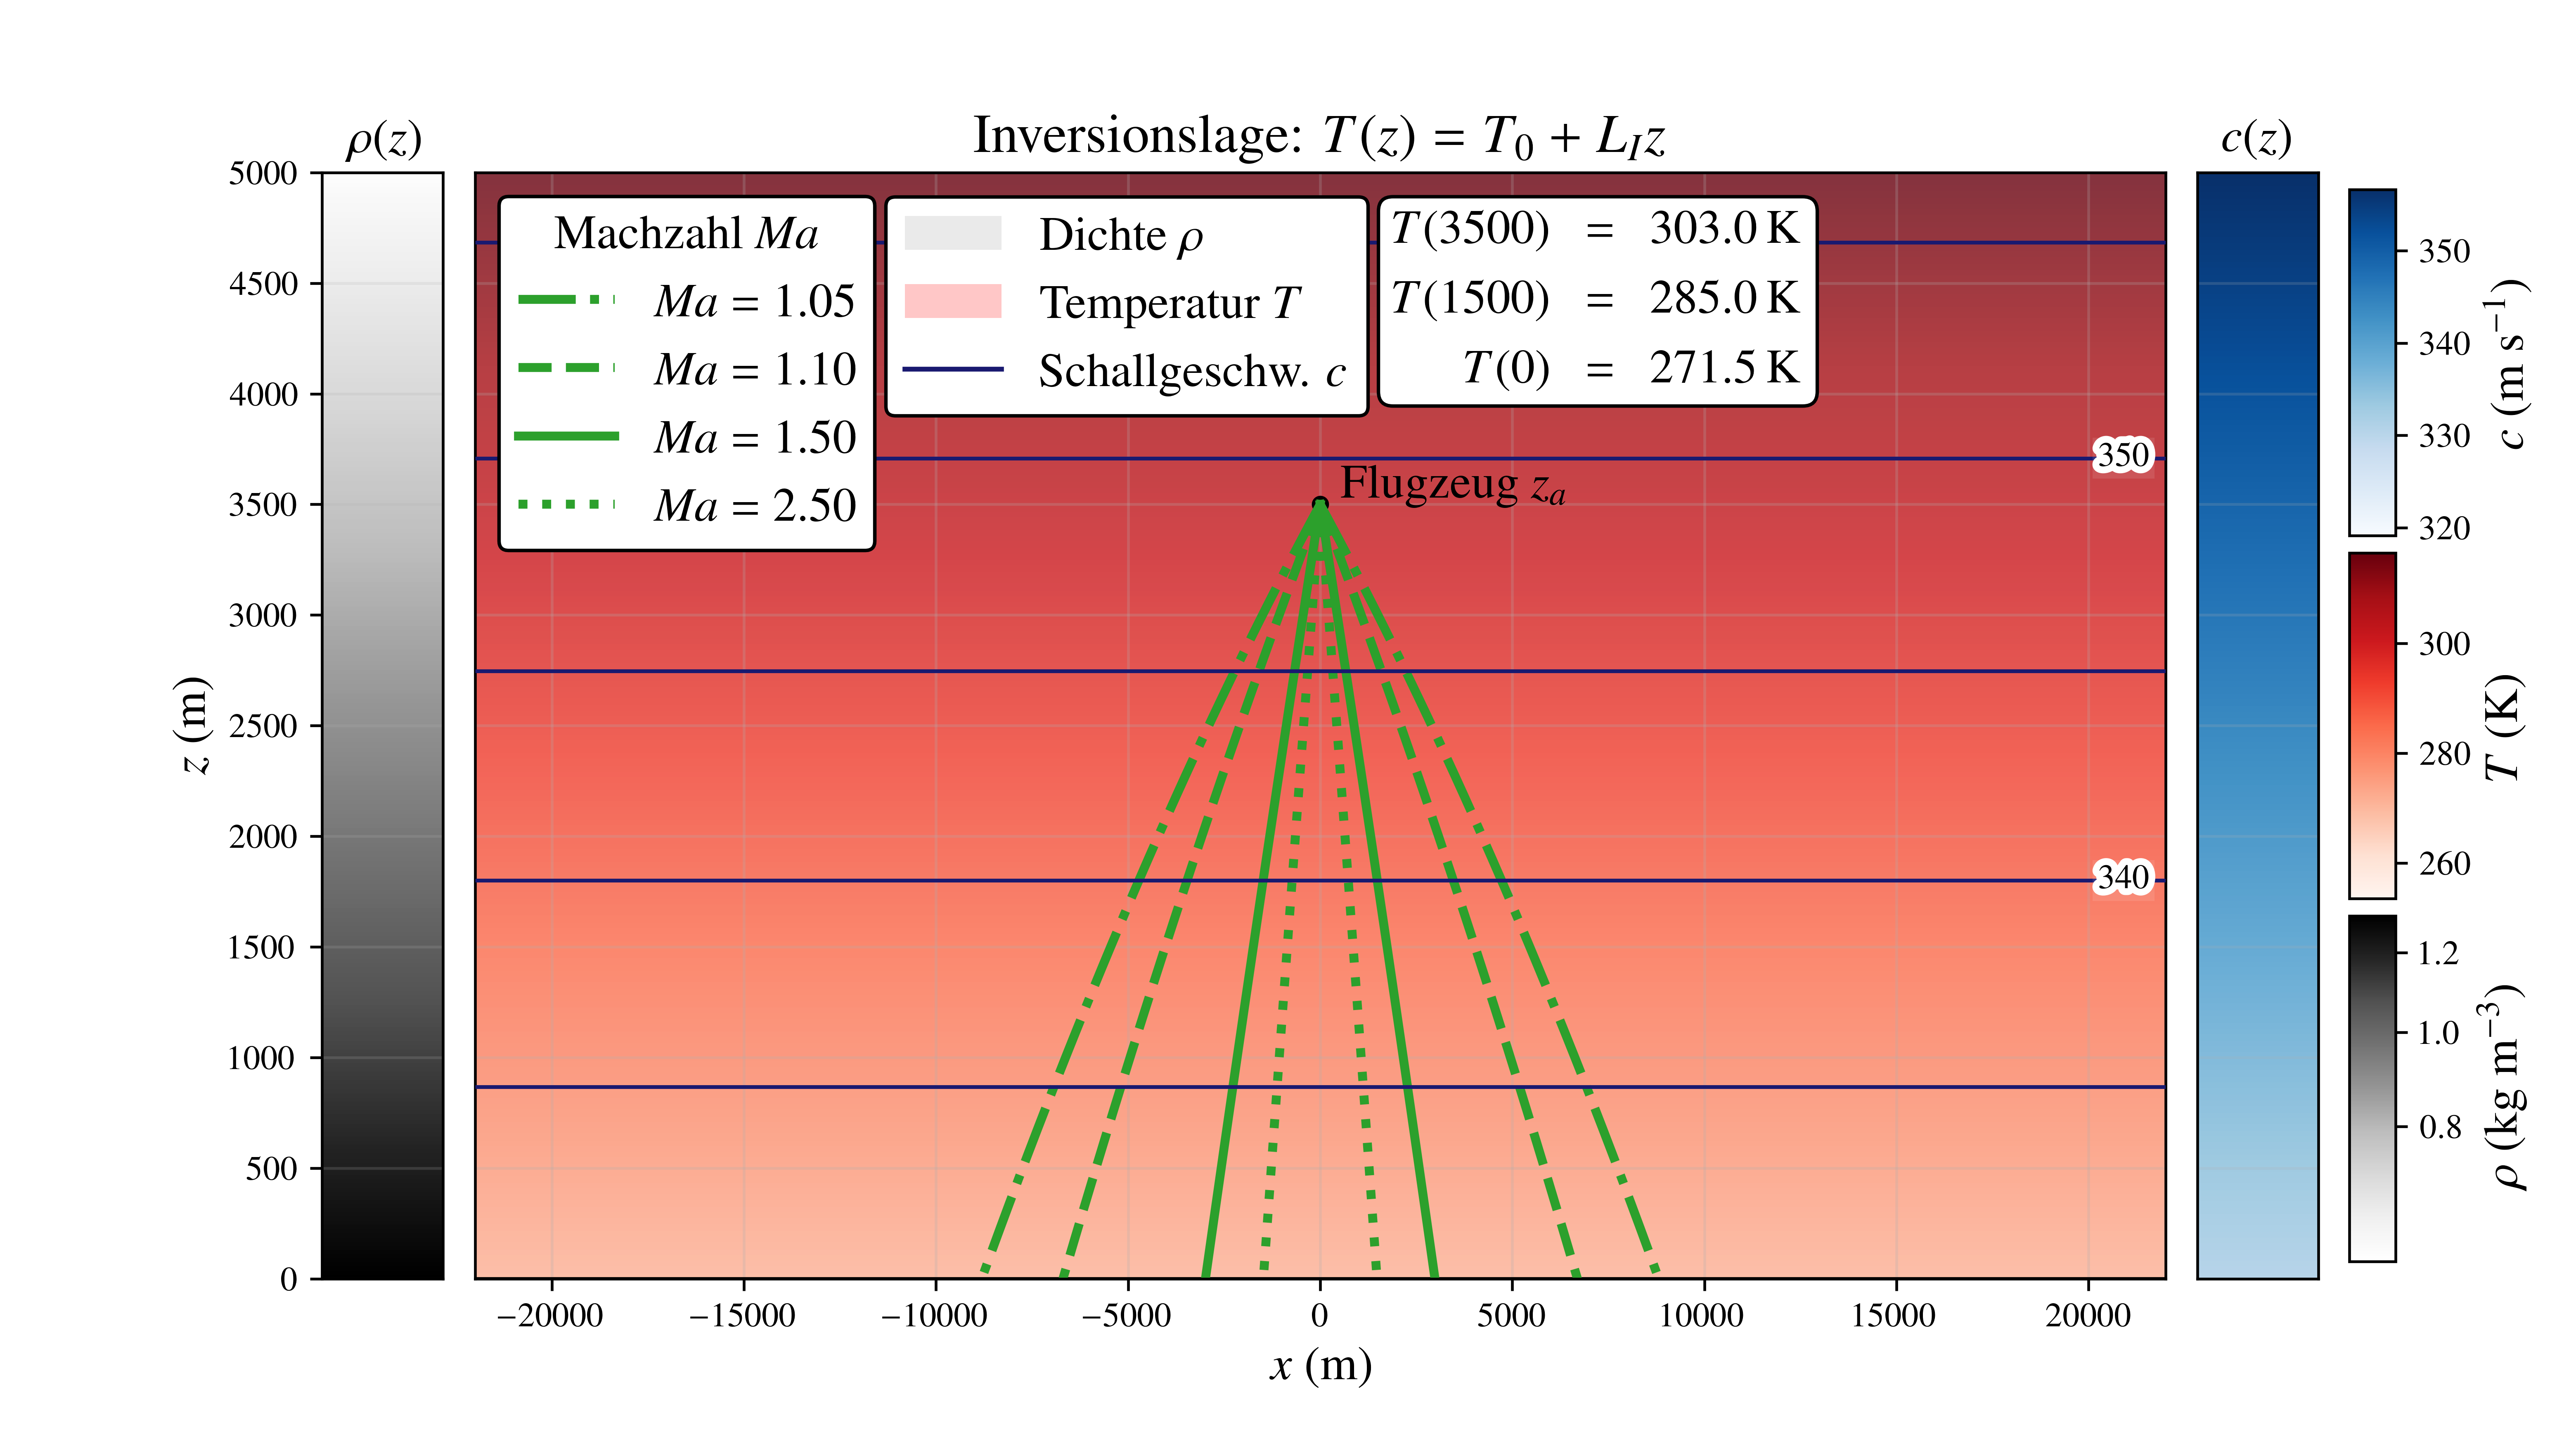
\includegraphics[width=0.9\linewidth]{papers/schall/figures/inversion_sidepanels.png}
%   \captionof{subfigure}{Inversionslage}
%   \label{fig:inv}
% \end{minipage}

% \vspace{\baselineskip}

% \begin{minipage}[t]{0.5\textwidth}
%   \centering
%   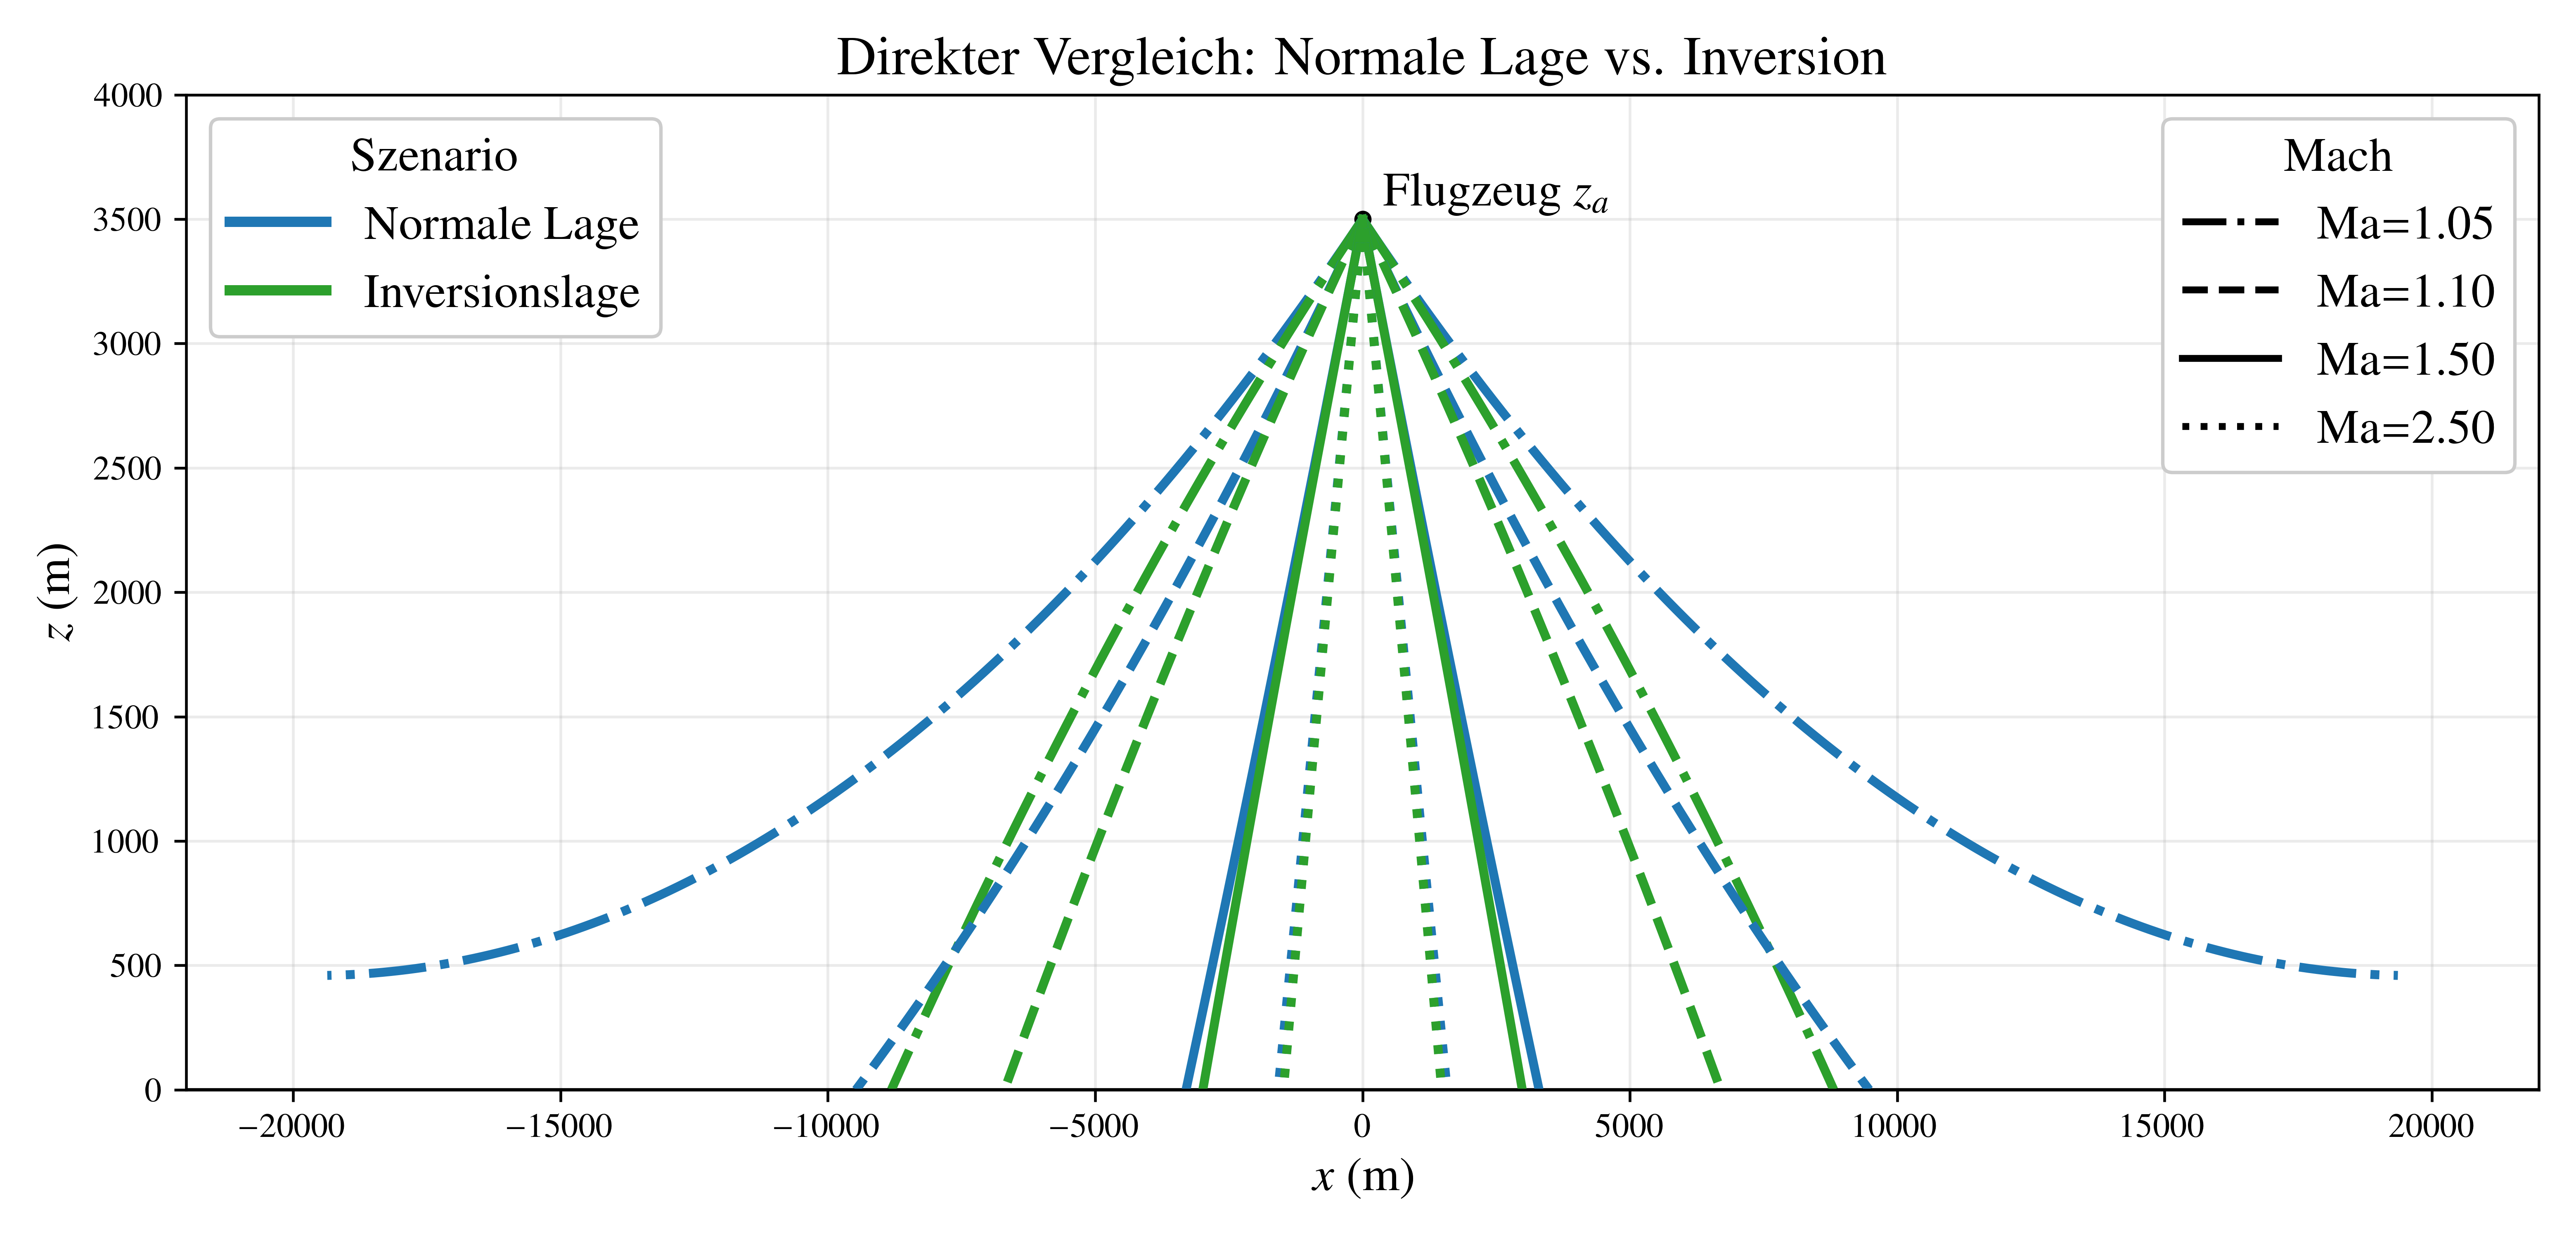
\includegraphics[width=0.9\linewidth]{papers/schall/figures/overlay_clean.png}
%   \captionof{subfigure}{Direkter Vergleich}
%   \label{fig:overlay}
% \end{minipage}

% \caption{Schallausbreitung für normale Lage, Inversionslage und für Wendepunkte.}
% \label{fig:schall:gesamt}
% \end{figure}

\begin{figure}
    \centering
    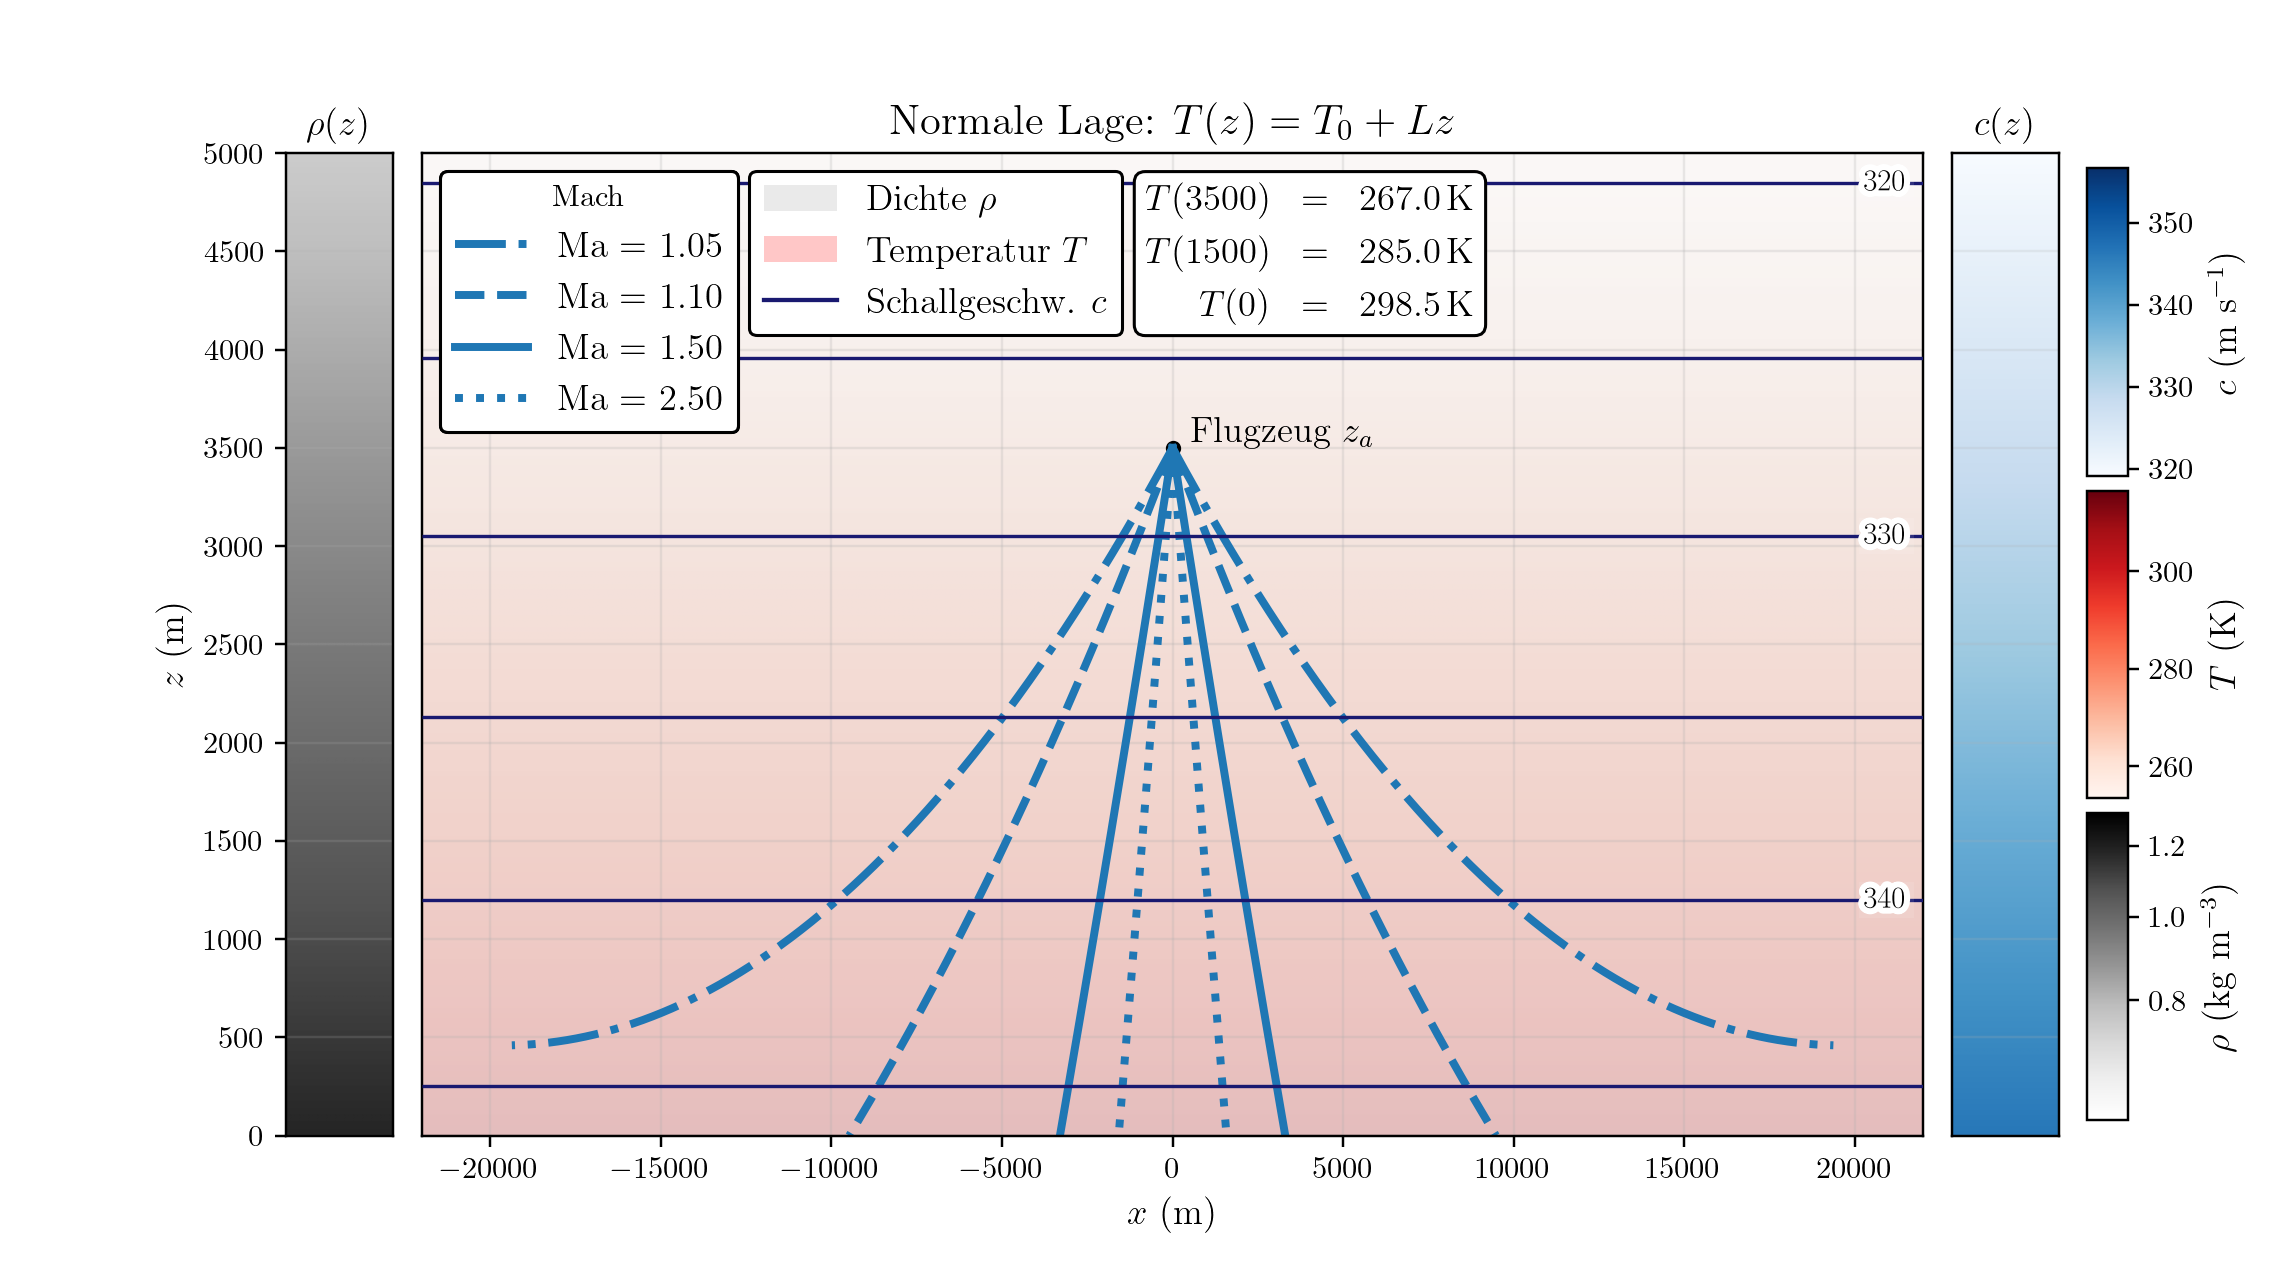
\includegraphics[width=\textwidth]{papers/schall/figures/normal_sidepanels.png}
    \caption{Schallausbreitung für normale Lage.}
    \label{fig:schall:norm-lage}
\end{figure}

\begin{figure}
    \centering
    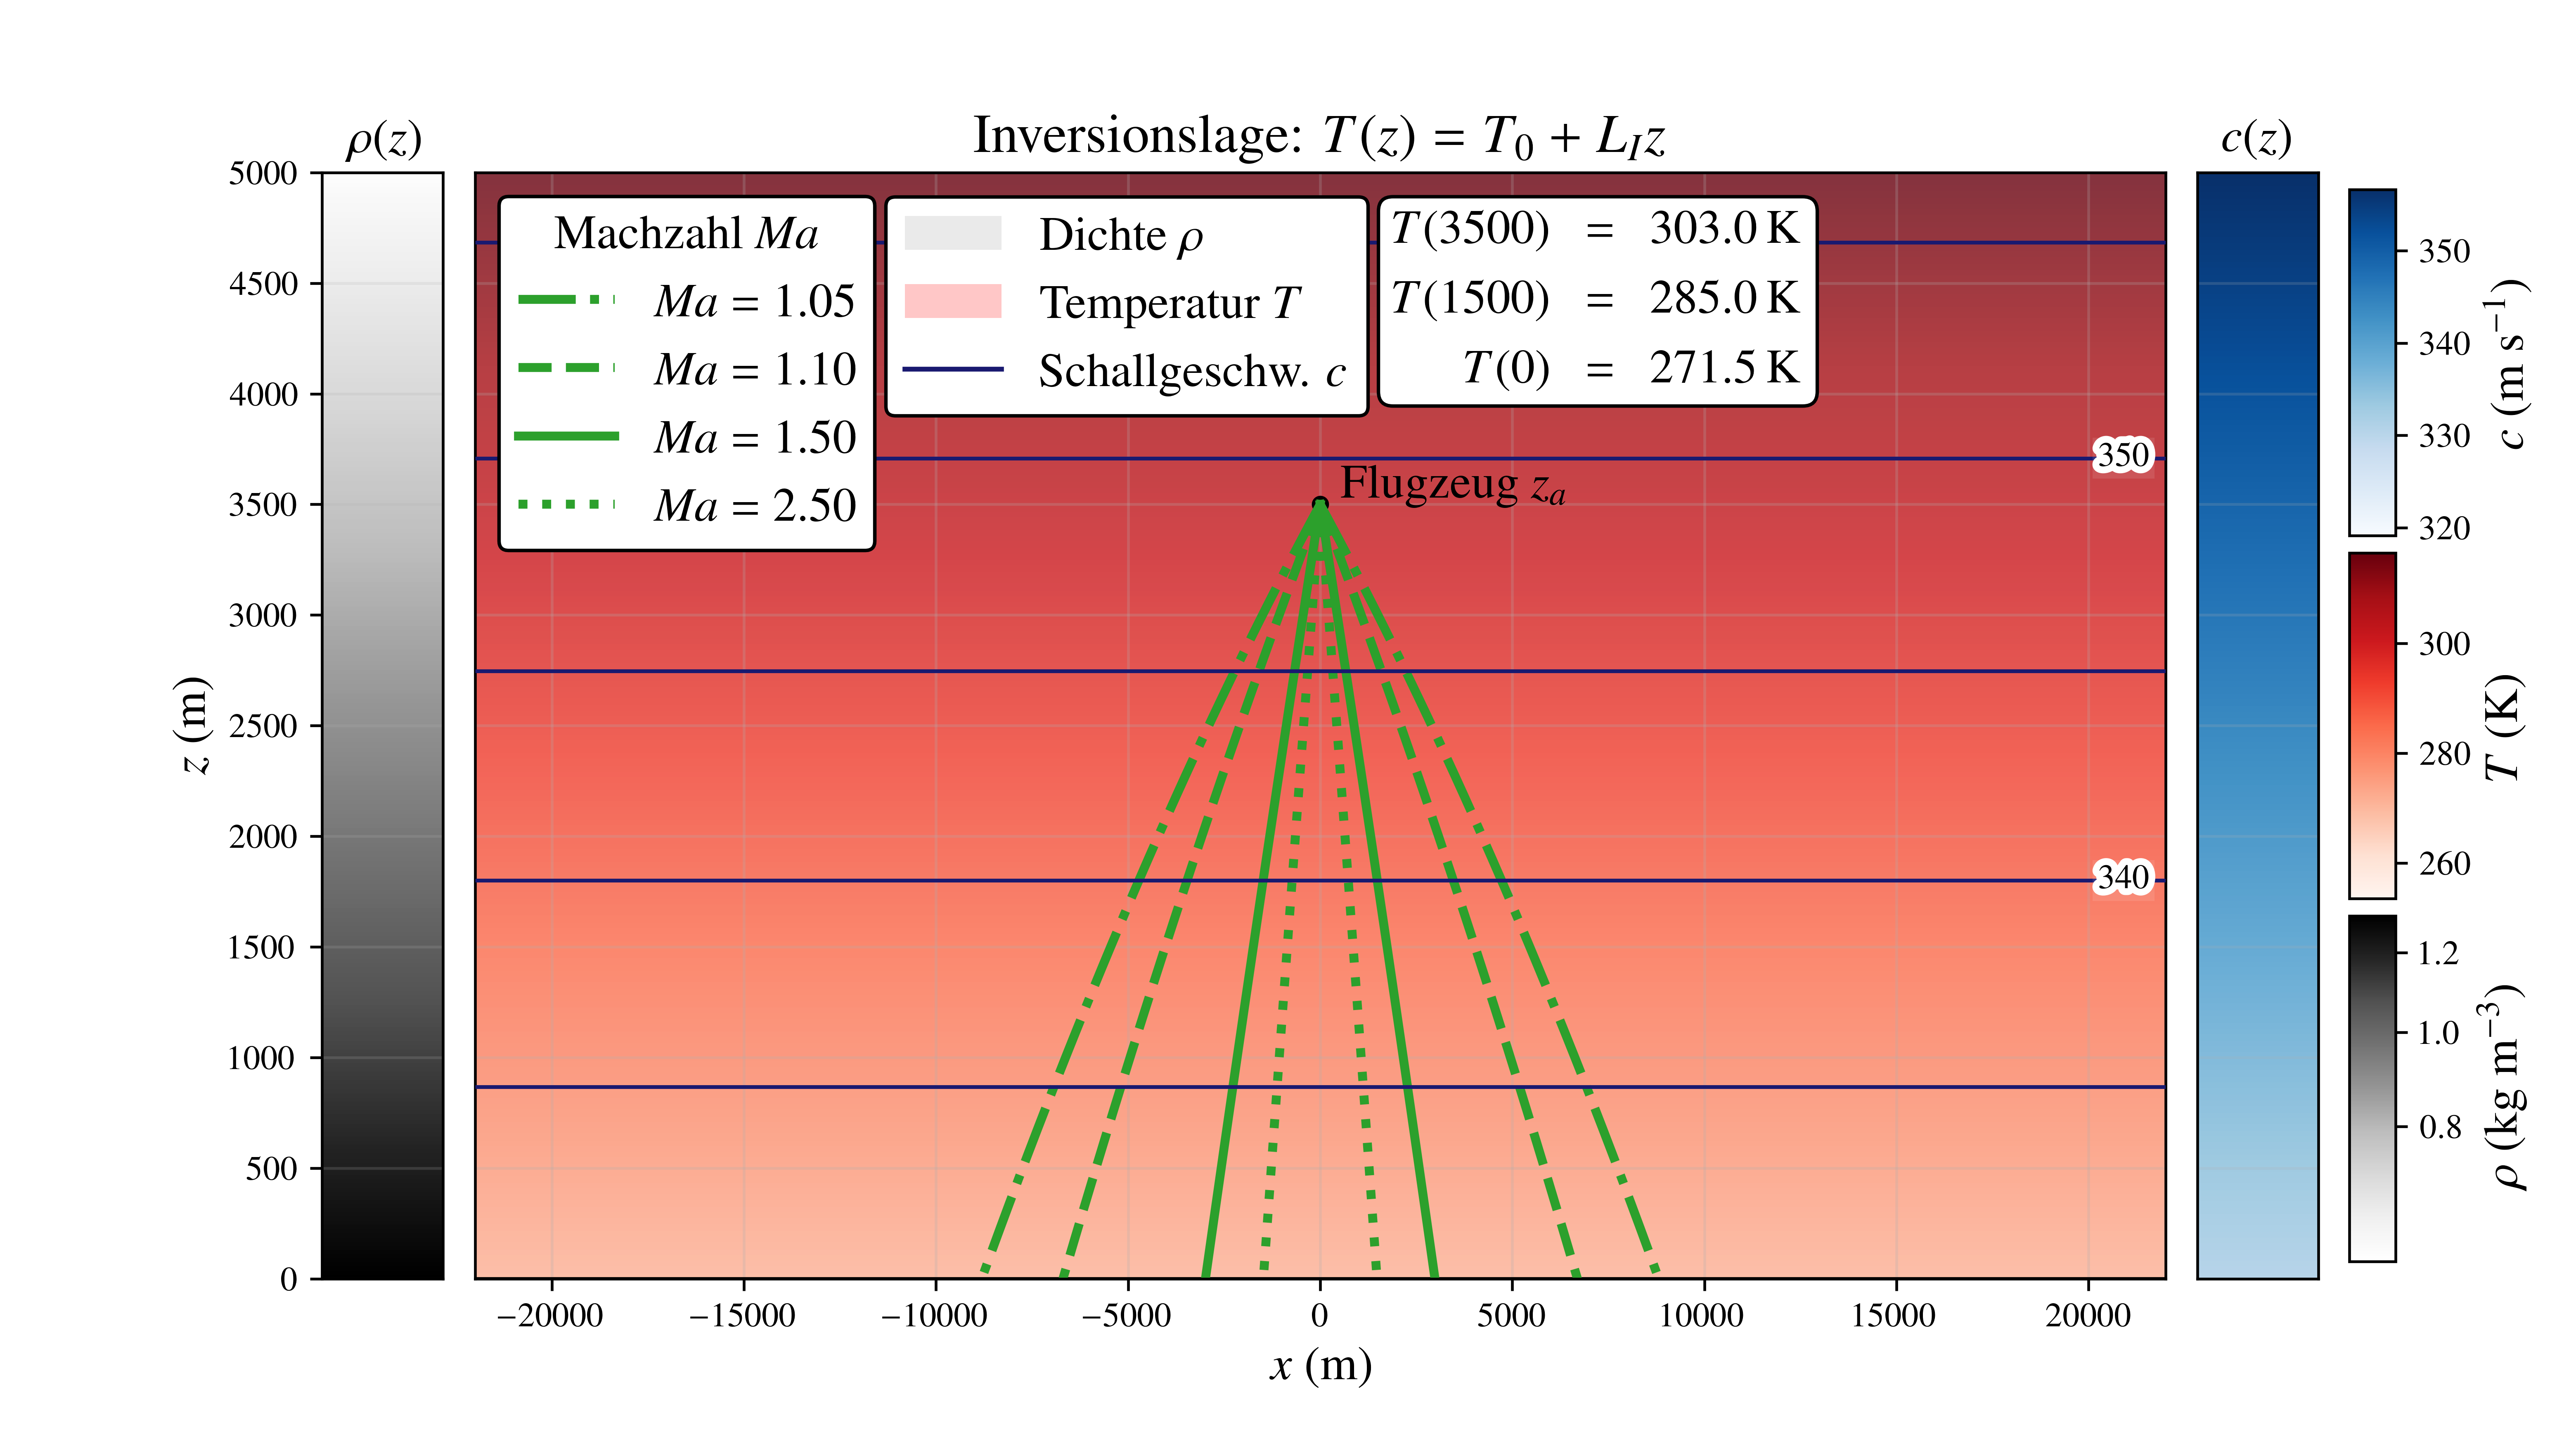
\includegraphics[width=\textwidth]{papers/schall/figures/inversion_sidepanels.png}
    \caption{Schallausbreitung für Inversionslage.}
    \label{fig:schall:inv-lage}
\end{figure}

\begin{figure}
    \centering
    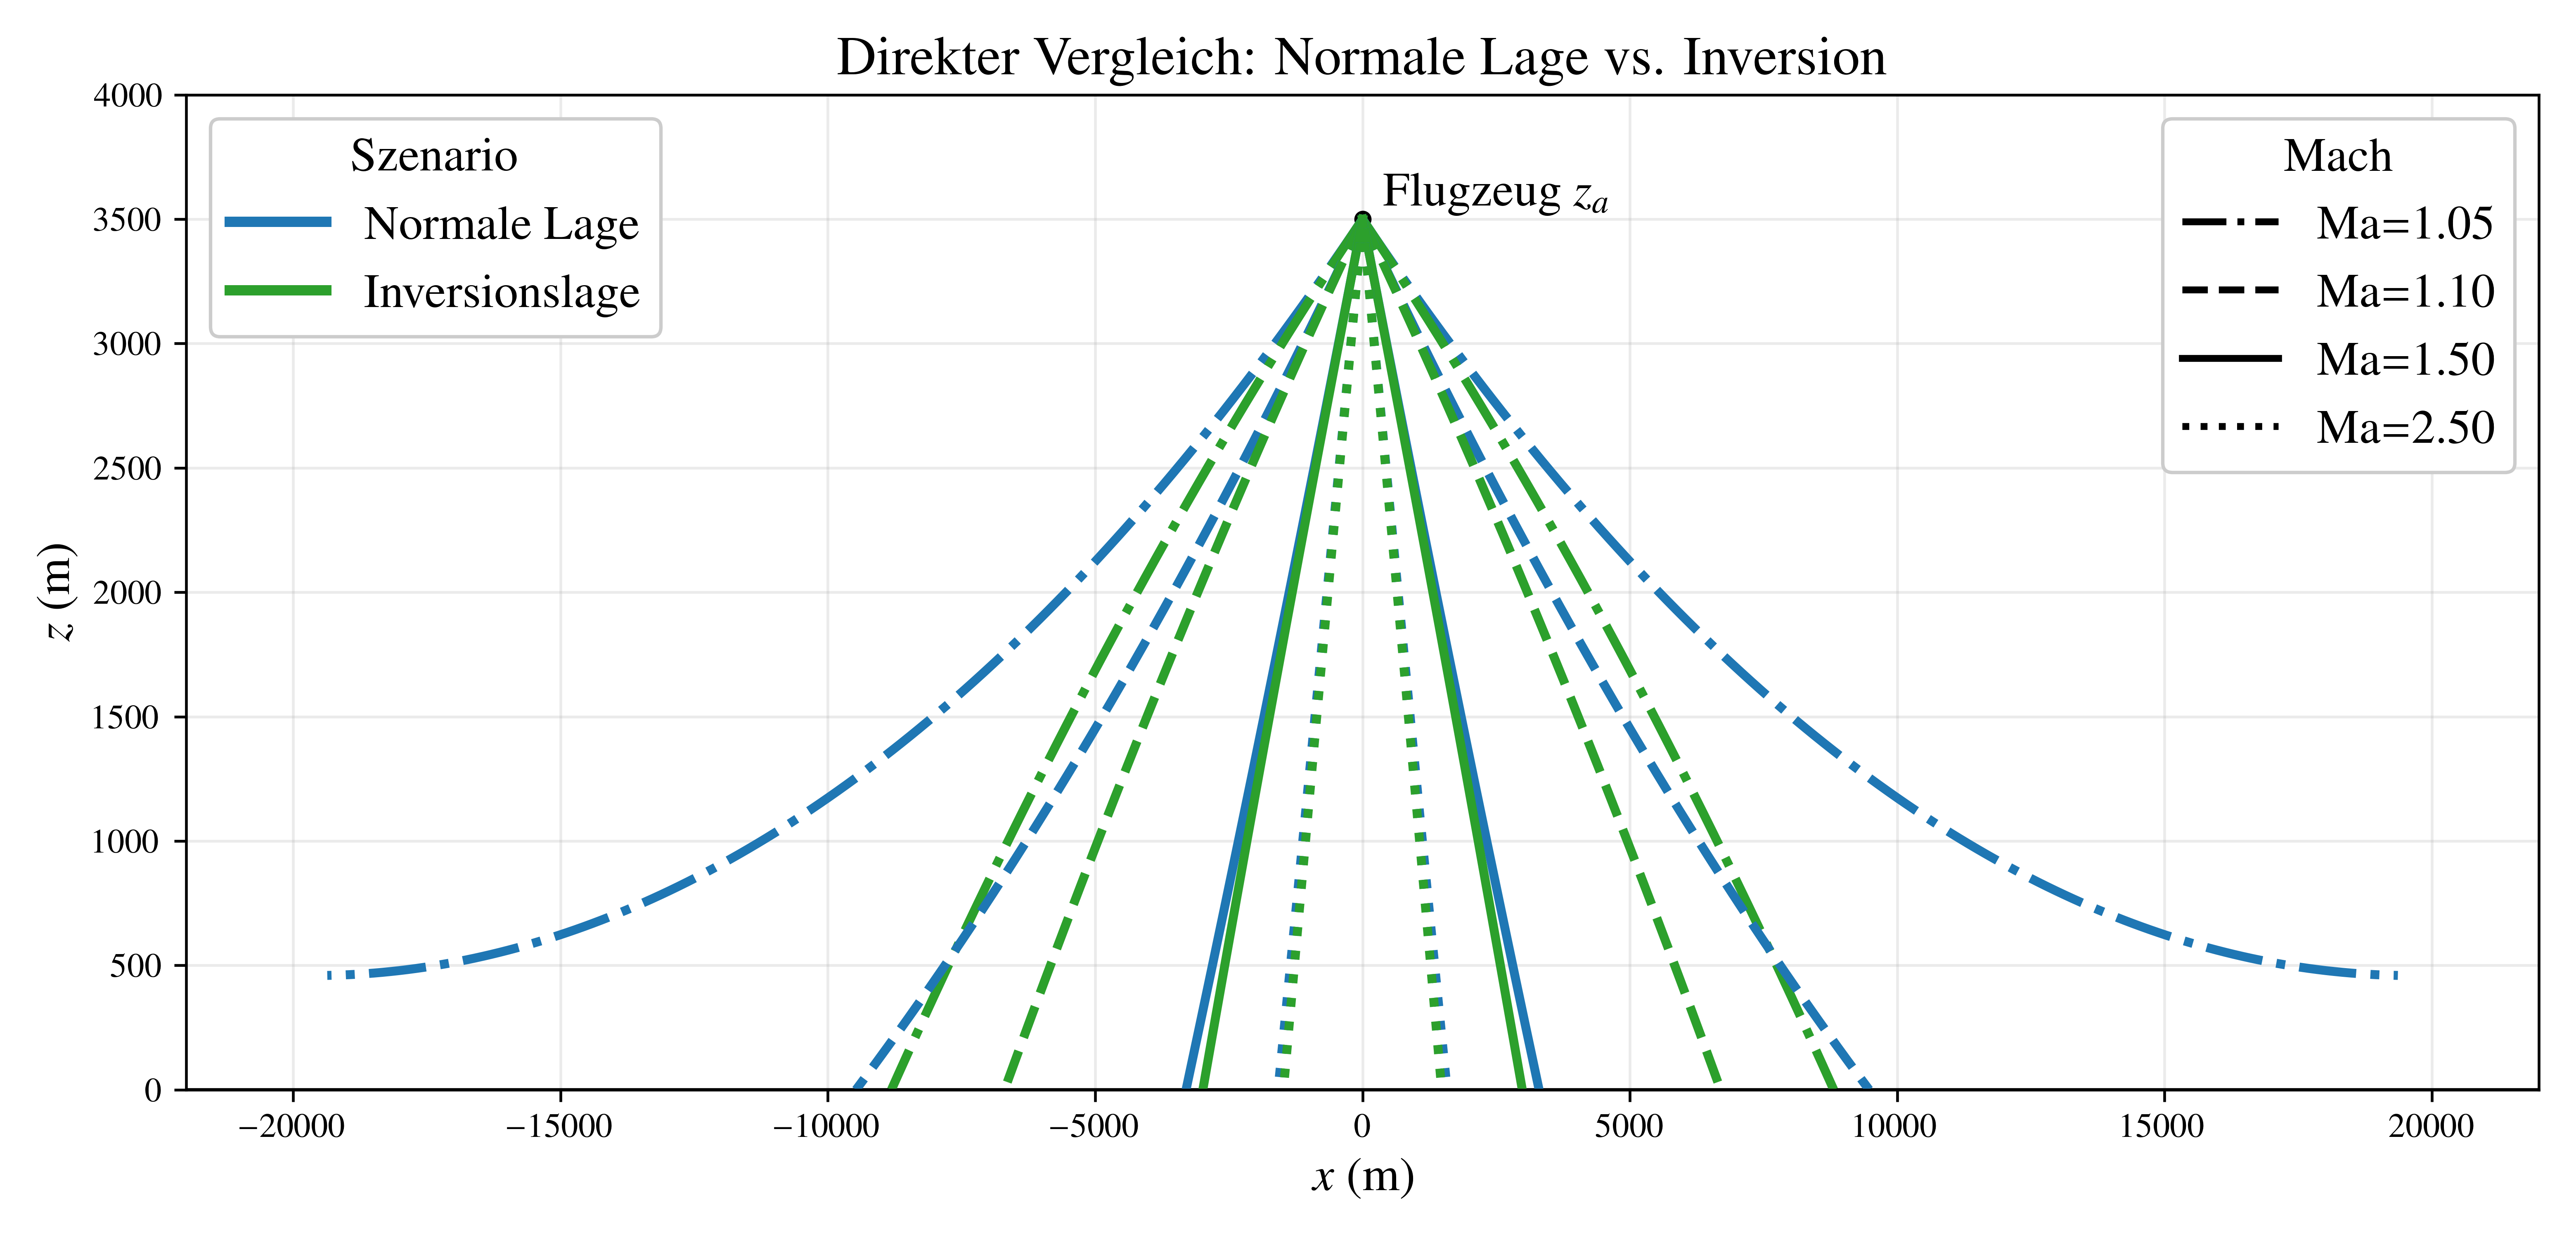
\includegraphics[width=\textwidth]{papers/schall/figures/overlay_clean.png}
    \caption{Schallausbreitung im direkter Vergleich.}
    \label{fig:schall:norm-vs-inv-lage}
\end{figure}